\chapter{Research Analysis and Methodology}

This chapter presents the formal mathematical foundations of the proposed RE-TabSyn framework, beginning with the problem formulation, proceeding through the theoretical basis of each baseline method, and culminating in a detailed description of our three-component architecture with accompanying theoretical analysis.

\section{Problem Formulation}

Let $\mathcal{D} = \{(\mathbf{x}_i, y_i)\}_{i=1}^{N}$ denote a tabular dataset where $\mathbf{x}_i \in \mathcal{X}$ represents a feature vector and $y_i \in \{0, 1\}$ denotes the class label.

Each feature vector comprises numerical and categorical attributes:
\begin{equation}
\mathbf{x} = (\mathbf{x}^{(num)}, \mathbf{x}^{(cat)}) \in \mathbb{R}^{d_{num}} \times \prod_{j=1}^{d_{cat}} \mathcal{C}_j
\end{equation}
where $\mathcal{C}_j$ is the categorical domain for attribute $j$ with cardinality $|\mathcal{C}_j|$.

The class imbalance is quantified by the minority ratio $\rho = N_1 / N$, where $N_1 = |\{i : y_i = 1\}|$ is the minority class count. In our benchmark datasets, $\rho$ ranges from 0.048 to 0.445.

The core learning objective is: learn a generative model $G_\theta$ that synthesizes samples $\tilde{\mathbf{x}} \sim p_\theta(\mathbf{x})$ indistinguishable from $\mathbf{x} \sim p_{data}(\mathbf{x})$, with the additional capability to control the class distribution $p_\theta(y)$ at generation time. This is a stricter objective than standard generative modeling: the target is samples whose class composition can be specified by the user after training, not merely realistic samples. Four criteria guide the framework design:
\begin{enumerate}
    \item Fidelity: $p_\theta(\mathbf{x}) \approx p_{data}(\mathbf{x})$ (distributional similarity), measured by the Kolmogorov-Smirnov, i.e., KS, statistic, where lower values indicate better fidelity.

    \item Utility: Classifiers trained on synthetic data perform comparably to those trained on real data, measured via the Train-on-Synthetic Test-on-Real, i.e., TSTR, protocol using AUC-ROC and F1-score.

    \item Privacy: Synthetic samples do not memorize training instances, measured by Distance to Closest Record, i.e., DCR, where higher values indicate stronger privacy.

    \item Controllability: User-specified class ratio $\pi = P(y=1)$ achievable without model retraining, measured by the deviation between target and achieved minority ratios.
\end{enumerate}

No previous method satisfies all four desiderata simultaneously. TabSyn satisfies the first three but not the fourth. CTGAN partially satisfies fidelity and utility but fails on privacy (weak DCR) and completely fails on controllability. RE-TabSyn is designed to satisfy all four, accepting a modest fidelity cost relative to TabSyn as the price of gaining controllability.

\section{Baseline Methods: Theoretical Foundations}

This section provides the mathematical foundations of the four baseline methods against which RE-TabSyn is evaluated; each method's limitations motivate specific design choices in the proposed approach.

\subsection{Generative adversarial networks (GANs)}

GANs \cite{goodfellow2014gan} formulate generative modeling as a two-player minimax game between a generator $G$ and discriminator $D$:
\begin{equation}
\min_G \max_D \mathcal{L}_{GAN}(G, D) = \mathbb{E}_{\mathbf{x} \sim p_{data}}[\log D(\mathbf{x})] + \mathbb{E}_{\mathbf{z} \sim p_z}[\log(1 - D(G(\mathbf{z})))]
\end{equation}

Training dynamics are notoriously unstable: a discriminator that is too strong causes vanishing gradients for $G$, while one that is too weak provides no learning signal. Techniques such as Wasserstein distance \cite{arjovsky2017wgan} and spectral normalization help, but do not fully resolve the problem.

CTGAN \cite{xu2019ctgan} extends vanilla GANs for tabular data through two innovations:
\begin{enumerate}
    \item Mode-specific normalization: numerical columns are modeled as mixtures of Gaussians via VGMMs, allowing the transform to adapt to multimodal distributions rather than assuming unimodal structure.

    \item Conditional generator with training-by-sampling: a conditional vector specifies which categorical value to generate, and training oversamples rare categories.
\end{enumerate}

Despite these innovations, CTGAN suffers from mode collapse on minority classes: the generator may ``forget'' rare modes because the gradient signal from minority samples is overwhelmed by the majority class signal. CTGAN also provides no mechanism for post-hoc ratio adjustment; the generated data mirrors the training distribution. In experiments on the Polish Bankruptcy dataset (4.8\% minority), CTGAN achieves a minority F1-score of just 0.112, barely above random guessing, confirming that mode collapse on extreme minority classes is a practical failure, not merely a theoretical concern.

\subsection{Variational autoencoders}

VAEs \cite{kingma2014vae} model data through latent variables $\mathbf{z}$ using variational inference. The core idea: instead of directly modeling the complicated high-dimensional data distribution $p(\mathbf{x})$, introduce a simpler latent variable $\mathbf{z}$ and model the joint distribution $p(\mathbf{x}, \mathbf{z})$. Generation then proceeds by first sampling $\mathbf{z} \sim p(\mathbf{z})$ from the simple prior (a standard Gaussian) and then decoding $\mathbf{x} \sim p_\theta(\mathbf{x}|\mathbf{z})$.

The generative model defines a joint distribution $p_\theta(\mathbf{x}, \mathbf{z}) = p_\theta(\mathbf{x}|\mathbf{z}) p(\mathbf{z})$, where $p(\mathbf{z}) = \mathcal{N}(\mathbf{0}, \mathbf{I})$ is a standard Gaussian prior. Since the true posterior is intractable, an approximate posterior $q_\phi(\mathbf{z}|\mathbf{x})$ is introduced. The Evidence Lower Bound, i.e., ELBO, provides a tractable training objective:
\begin{equation}
\log p_\theta(\mathbf{x}) \geq \underbrace{\mathbb{E}_{q_\phi(\mathbf{z}|\mathbf{x})}[\log p_\theta(\mathbf{x}|\mathbf{z})]}_{\text{Reconstruction Term}} - \underbrace{D_{KL}(q_\phi(\mathbf{z}|\mathbf{x}) \parallel p(\mathbf{z}))}_{\text{Regularization Term}}
\end{equation}

The reconstruction term encourages the encoder to produce informative latent codes. The KL term regularizes the posterior toward the Gaussian prior.

The reparameterization trick $\mathbf{z} = \boldsymbol{\mu} + \boldsymbol{\sigma} \odot \boldsymbol{\epsilon}$, where $\boldsymbol{\epsilon} \sim \mathcal{N}(\mathbf{0}, \mathbf{I})$, enables end-to-end gradient-based optimization.

TVAE applies VAE principles to tabular data with mixed-type reconstruction losses (MSE for numerical features, cross-entropy for categorical features) but has three limitations. First, the Gaussian likelihood assumption produces blurry reconstructions that average over modes rather than capturing them sharply, potentially generating unrealistic in-between samples. Second, in high-dimensional settings the KL term can dominate training, causing posterior collapse where the decoder learns to reconstruct without using the latent code. Third, TVAE has no class conditioning mechanism, preventing controlled generation.

RE-TabSyn addresses these limitations by using a $\beta$-VAE formulation ($\beta = 0.1$, weighting the KL term down) to prevent posterior collapse while maintaining smooth latent geometry, and by adding class conditioning through the downstream diffusion model rather than into the VAE itself.

\subsection{Diffusion models}

Diffusion models \cite{ho2020ddpm} define a forward noising process that gradually destroys data structure, and then learn to reverse it. The intuition is straightforward: if you know how data is destroyed, you can learn to reconstruct it.

The forward process is a Markov chain that adds Gaussian noise over $T$ timesteps according to a variance schedule $\{\beta_t\}_{t=1}^{T}$:
\begin{equation}
q(\mathbf{z}_t | \mathbf{z}_{t-1}) = \mathcal{N}(\mathbf{z}_t; \sqrt{1-\beta_t}\,\mathbf{z}_{t-1}, \beta_t \mathbf{I})
\end{equation}

A useful property enables direct sampling of any timestep $t$ without iterating through all previous steps:
\begin{equation}
q(\mathbf{z}_t | \mathbf{z}_0) = \mathcal{N}(\mathbf{z}_t; \sqrt{\bar{\alpha}_t}\,\mathbf{z}_0, (1-\bar{\alpha}_t)\mathbf{I})
\end{equation}
where $\alpha_t = 1 - \beta_t$ and $\bar{\alpha}_t = \prod_{s=1}^{t} \alpha_s$.

The reverse process learns to denoise by predicting the noise $\epsilon_\theta(\mathbf{z}_t, t)$ added at each step, trained with a simple MSE objective:
\begin{equation}
\mathcal{L}_{simple} = \mathbb{E}_{t, \mathbf{z}_0, \boldsymbol{\epsilon}} \left[ \|\boldsymbol{\epsilon} - \epsilon_\theta(\mathbf{z}_t, t)\|^2 \right]
\end{equation}

\begin{figure}[H]
\centering
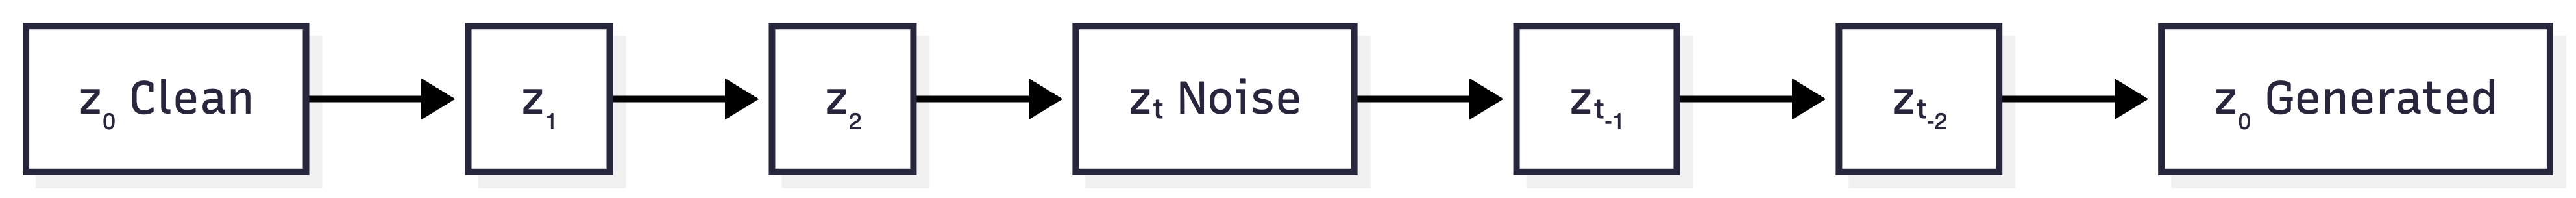
\includegraphics[width=\textwidth]{img/diffusion_chain.png}
\caption{Forward and reverse diffusion process.}
\label{fig:diffusion_chain}
\end{figure}

TabDDPM \cite{kotelnikov2023tabddpm} was the first systematic application of diffusion to tabular data. It treats numerical features with Gaussian diffusion and categorical features with multinomial diffusion. However, it demonstrates poor performance on mixed-type data because direct diffusion on one-hot encoded categorical features creates sparse, discontinuous gradients. To see why: a one-hot vector like $[0, 0, 1, 0]$ has most values at exactly zero. Adding Gaussian noise produces a dense vector like $[0.05, -0.12, 0.88, 0.03]$ that does not correspond to any valid category. The model must denoise vectors it has never seen in training data, creating a mismatch between the training distribution and the inference distribution. Our experiments confirm this failure: TabDDPM achieves an average KS statistic of 0.770, indicating near-complete distributional mismatch.

TabSyn \cite{zhang2024tabsyn} addresses TabDDPM's limitations by performing diffusion in a learned latent space. A VAE first encodes mixed-type tabular data into continuous representations where diffusion operates effectively. The discrete categorical values are absorbed into the continuous latent space by the VAE encoder, so the diffusion model only ever sees continuous vectors. A Transformer backbone then captures inter-column dependencies, achieving the best reported tabular fidelity at the time with an average KS of 0.109. However, TabSyn lacks any mechanism for controlling class distribution and cannot address class imbalance explicitly.

\section{Proposed Method: RE-TabSyn}

RE-TabSyn (Rare-Event Enhanced Tabular Synthesis) combines three interlocking components to achieve both fidelity and controllable minority generation. The complete system architecture is illustrated in Figure~\ref{fig:system_architecture}.

\begin{figure}[H]
\centering
\includegraphics[width=\textwidth]{img/system_architecture.png}
\caption{RE-TabSyn five-module system architecture.}
\label{fig:system_architecture}
\end{figure}

The three core components are:
\begin{enumerate}
    \item Variational Autoencoder (VAE) --- mixed-type encoding into continuous latent space
    \item Latent Diffusion Model (LDM) --- generation in the smooth continuous latent space
    \item Classifier-Free Guidance (CFG) --- controllable class ratios at inference time
\end{enumerate}

The three components are not independently useful; they work because of how they interact. The VAE solves the encoding problem so that the diffusion model operates in a well-behaved continuous space. The diffusion model learns a powerful generative model of that space. And the CFG mechanism uses the diffusion model's conditioning architecture to steer generation toward the desired class. Remove any one component and the system breaks: without the VAE, diffusion fails on categorical features; without the diffusion model, there is no way to apply CFG; without CFG, class control is impossible.

\subsection{Component 1: Tabular VAE}

The VAE is the foundation of RE-TabSyn, solving the critical problem of encoding heterogeneous tabular data into a smooth, continuous latent space where diffusion can operate effectively. The architecture is illustrated in Figure~\ref{fig:vae_architecture}.

\begin{figure}[H]
\centering
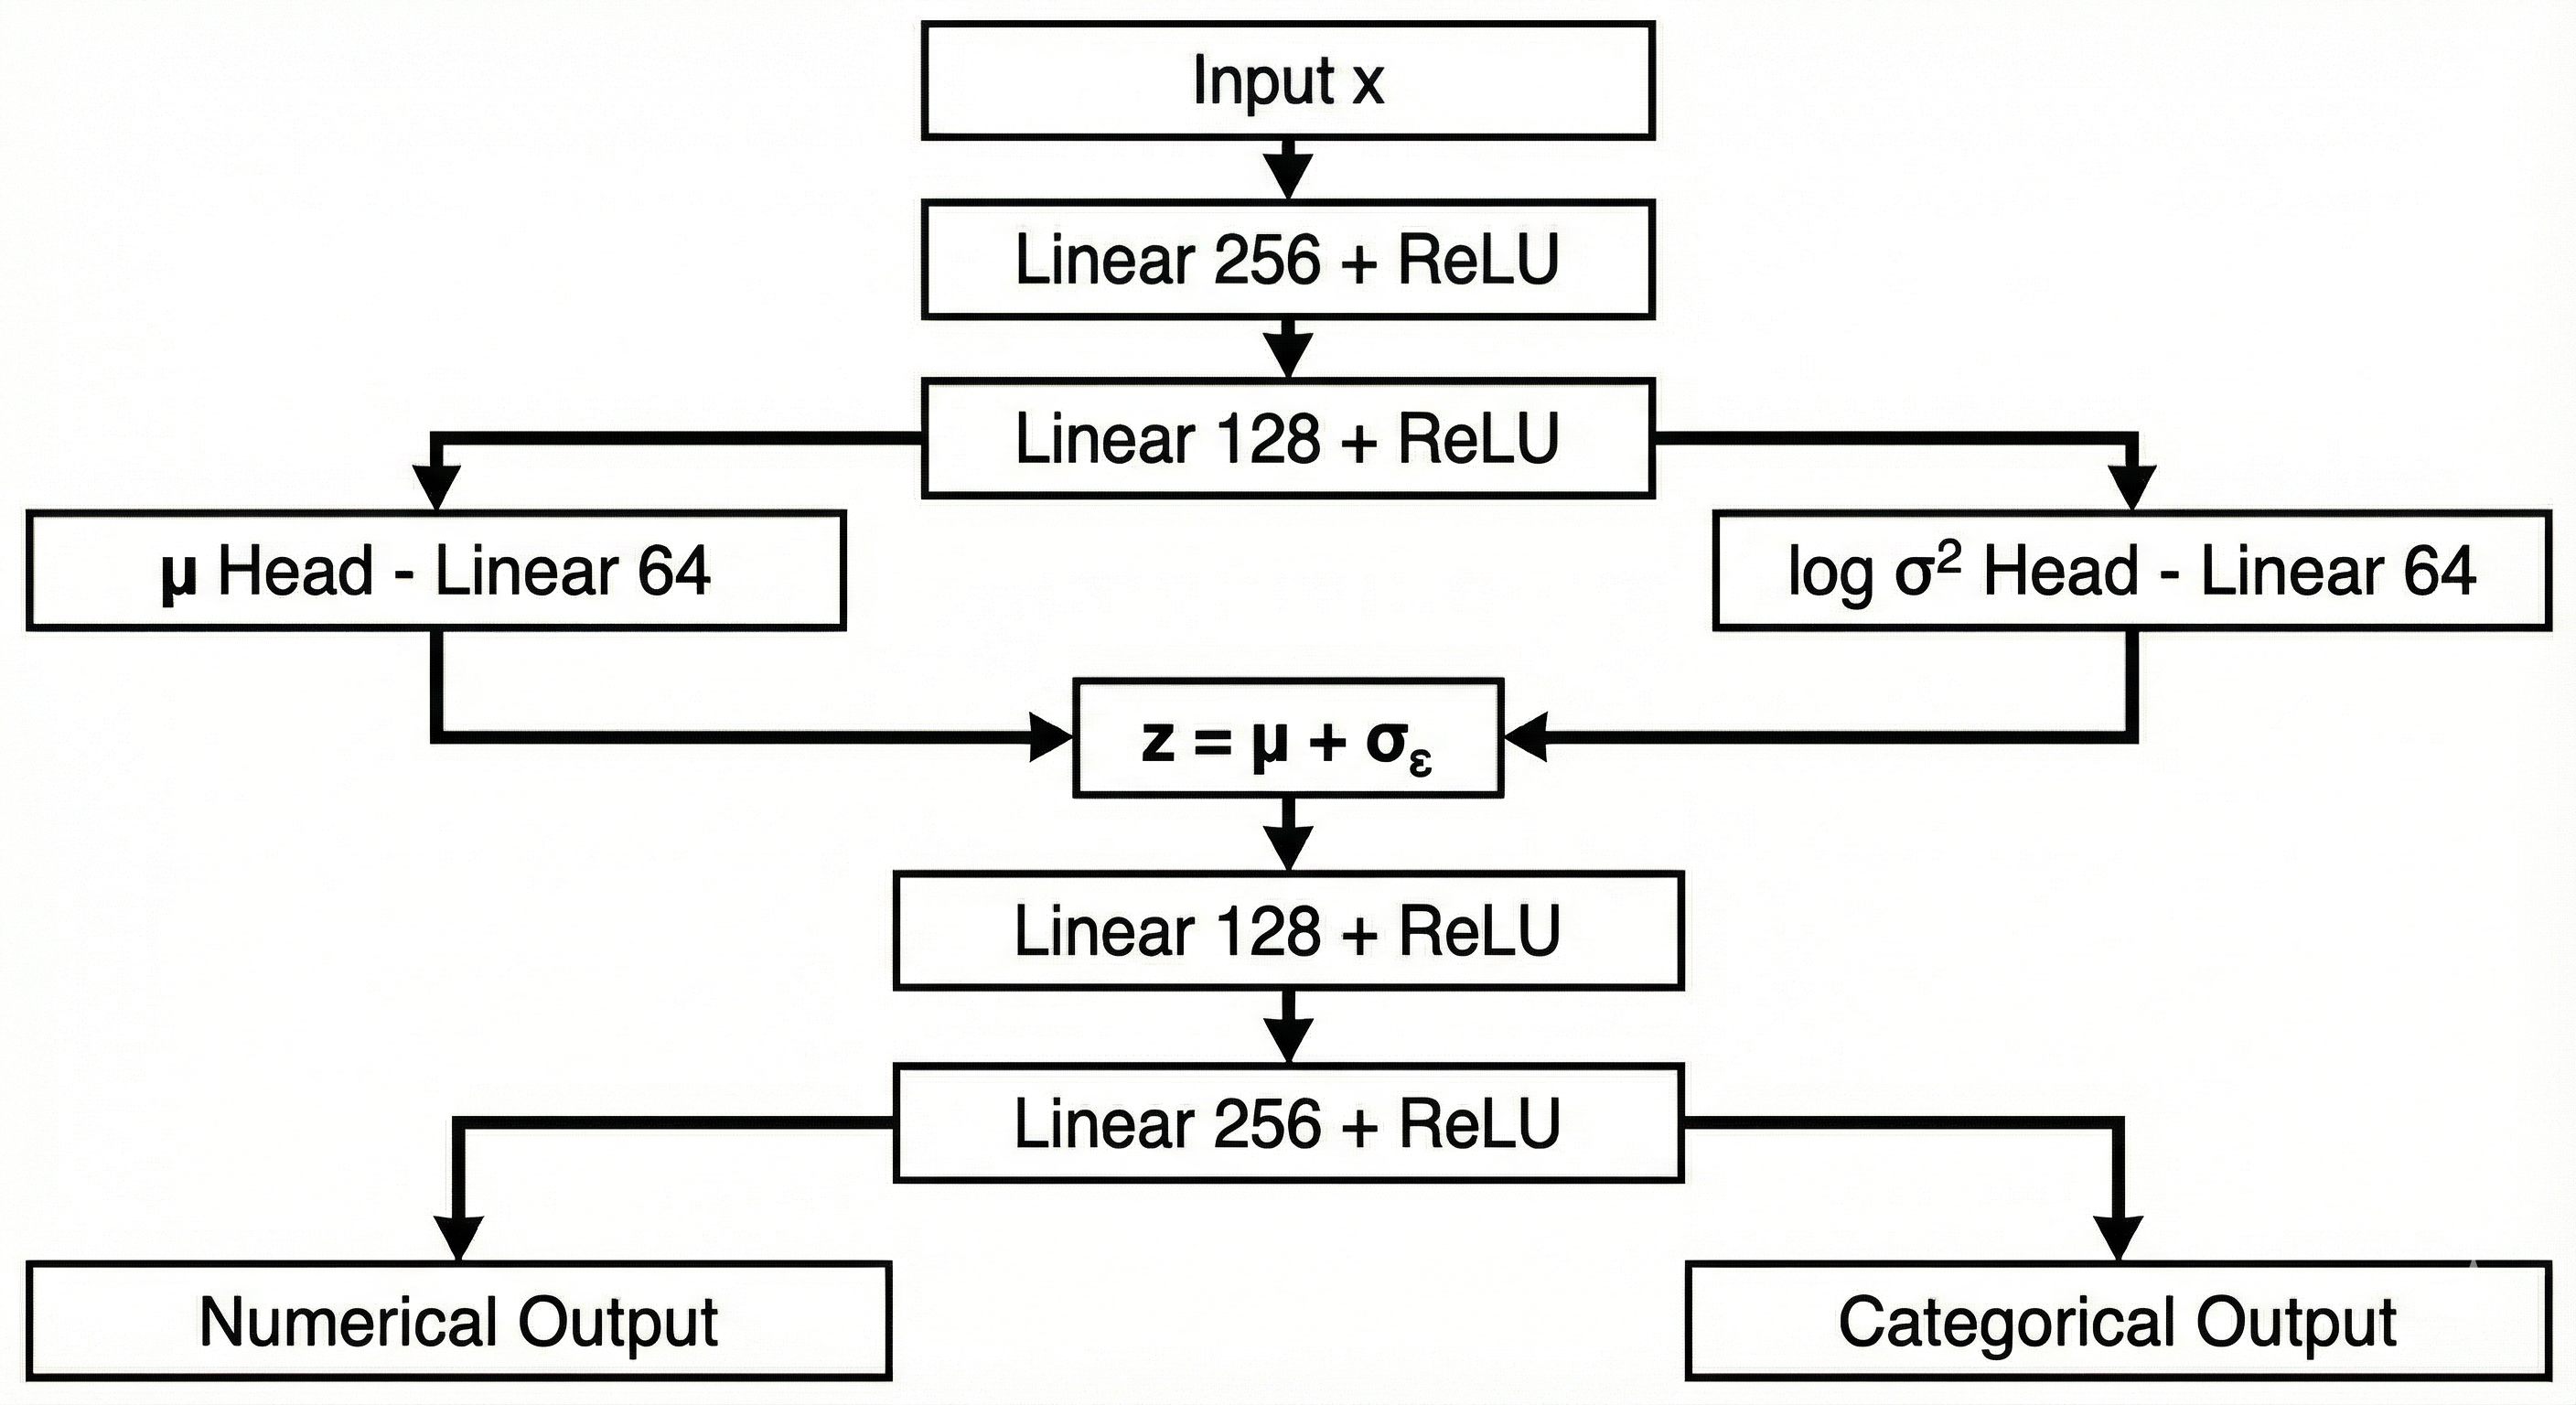
\includegraphics[width=0.85\textwidth]{img/vae_architecture.png}
\caption{Tabular VAE encoder-decoder architecture.}
\label{fig:vae_architecture}
\end{figure}

The encoder maps mixed-type input $\mathbf{x} \in \mathbb{R}^{d}$ to latent parameters $(\boldsymbol{\mu}, \log \boldsymbol{\sigma}^2)$ through an MLP with hidden dimensions (256, 128):
\begin{equation}
\boldsymbol{\mu}, \log \boldsymbol{\sigma}^2 = \text{Encoder}_\phi(\mathbf{x}) \quad \text{where} \quad \boldsymbol{\mu}, \log \boldsymbol{\sigma}^2 \in \mathbb{R}^{64}
\end{equation}

The latent variable is sampled via the reparameterization trick:
\begin{equation}
\mathbf{z} = \boldsymbol{\mu} + \boldsymbol{\sigma} \odot \boldsymbol{\epsilon}, \quad \boldsymbol{\epsilon} \sim \mathcal{N}(\mathbf{0}, \mathbf{I})
\end{equation}

Here, $\boldsymbol{\sigma} = \exp(\frac{1}{2} \log \boldsymbol{\sigma}^2)$ (computed element-wise), and $\odot$ denotes element-wise multiplication.

The decoder reconstructs from the latent code, utilizing separate loss functions for different feature types:
\begin{equation}
\mathcal{L}_{VAE} = \underbrace{\sum_{j=1}^{d_{num}} \|\mathbf{x}_j - \hat{\mathbf{x}}_j\|^2}_{\text{Numerical MSE}} + \underbrace{\sum_{j=1}^{d_{cat}} \text{CE}(\mathbf{x}_j, \hat{\mathbf{x}}_j)}_{\text{Categorical Cross-Entropy}} + \underbrace{\beta \cdot D_{KL}(q_\phi(\mathbf{z}|\mathbf{x}) \parallel p(\mathbf{z}))}_{\text{KL Regularization}}
\end{equation}
where $\beta = 0.1$ balances reconstruction quality and latent space regularization.

MSE is used for numerical features and cross-entropy for categorical features, since MSE is inappropriate for discrete class labels. $\beta = 0.1$ prevents posterior collapse while maintaining sufficient latent space regularity.

\subsection{Component 2: Latent diffusion model}

Given the encoded latent representation $\mathbf{z}_0 = \text{Encoder}_\phi(\mathbf{x})$, the forward diffusion process adds noise according to a linear schedule with $T = 1000$ timesteps, $\beta_1 = 10^{-4}$, and $\beta_T = 0.02$.

We employ a Diffusion Transformer (DiT) \cite{peebles2023dit} architecture for the noise prediction network, chosen for its ability to capture inter-feature dependencies through self-attention:
\begin{equation}
\epsilon_\theta(\mathbf{z}_t, t, y) = \text{DiT}(\mathbf{z}_t, \text{TimeEmb}(t), \text{ClassEmb}(y))
\end{equation}

The DiT architecture consists of:
\begin{enumerate}
    \item 4 Transformer layers with self-attention and feed-forward blocks.

    \item Hidden dimension of 256 with 4 attention heads (64 dimensions per head).

    \item Sinusoidal time embeddings projected through an MLP to match the hidden dimension.

    \item Learned class embeddings for the binary label (class 0, class 1, and null token $\emptyset$).

    \item Adaptive Layer Normalization (AdaLN) \cite{ba2016layernorm} conditioning each transformer block on the sum of time and class embeddings.
\end{enumerate}

\begin{figure}[H]
\centering
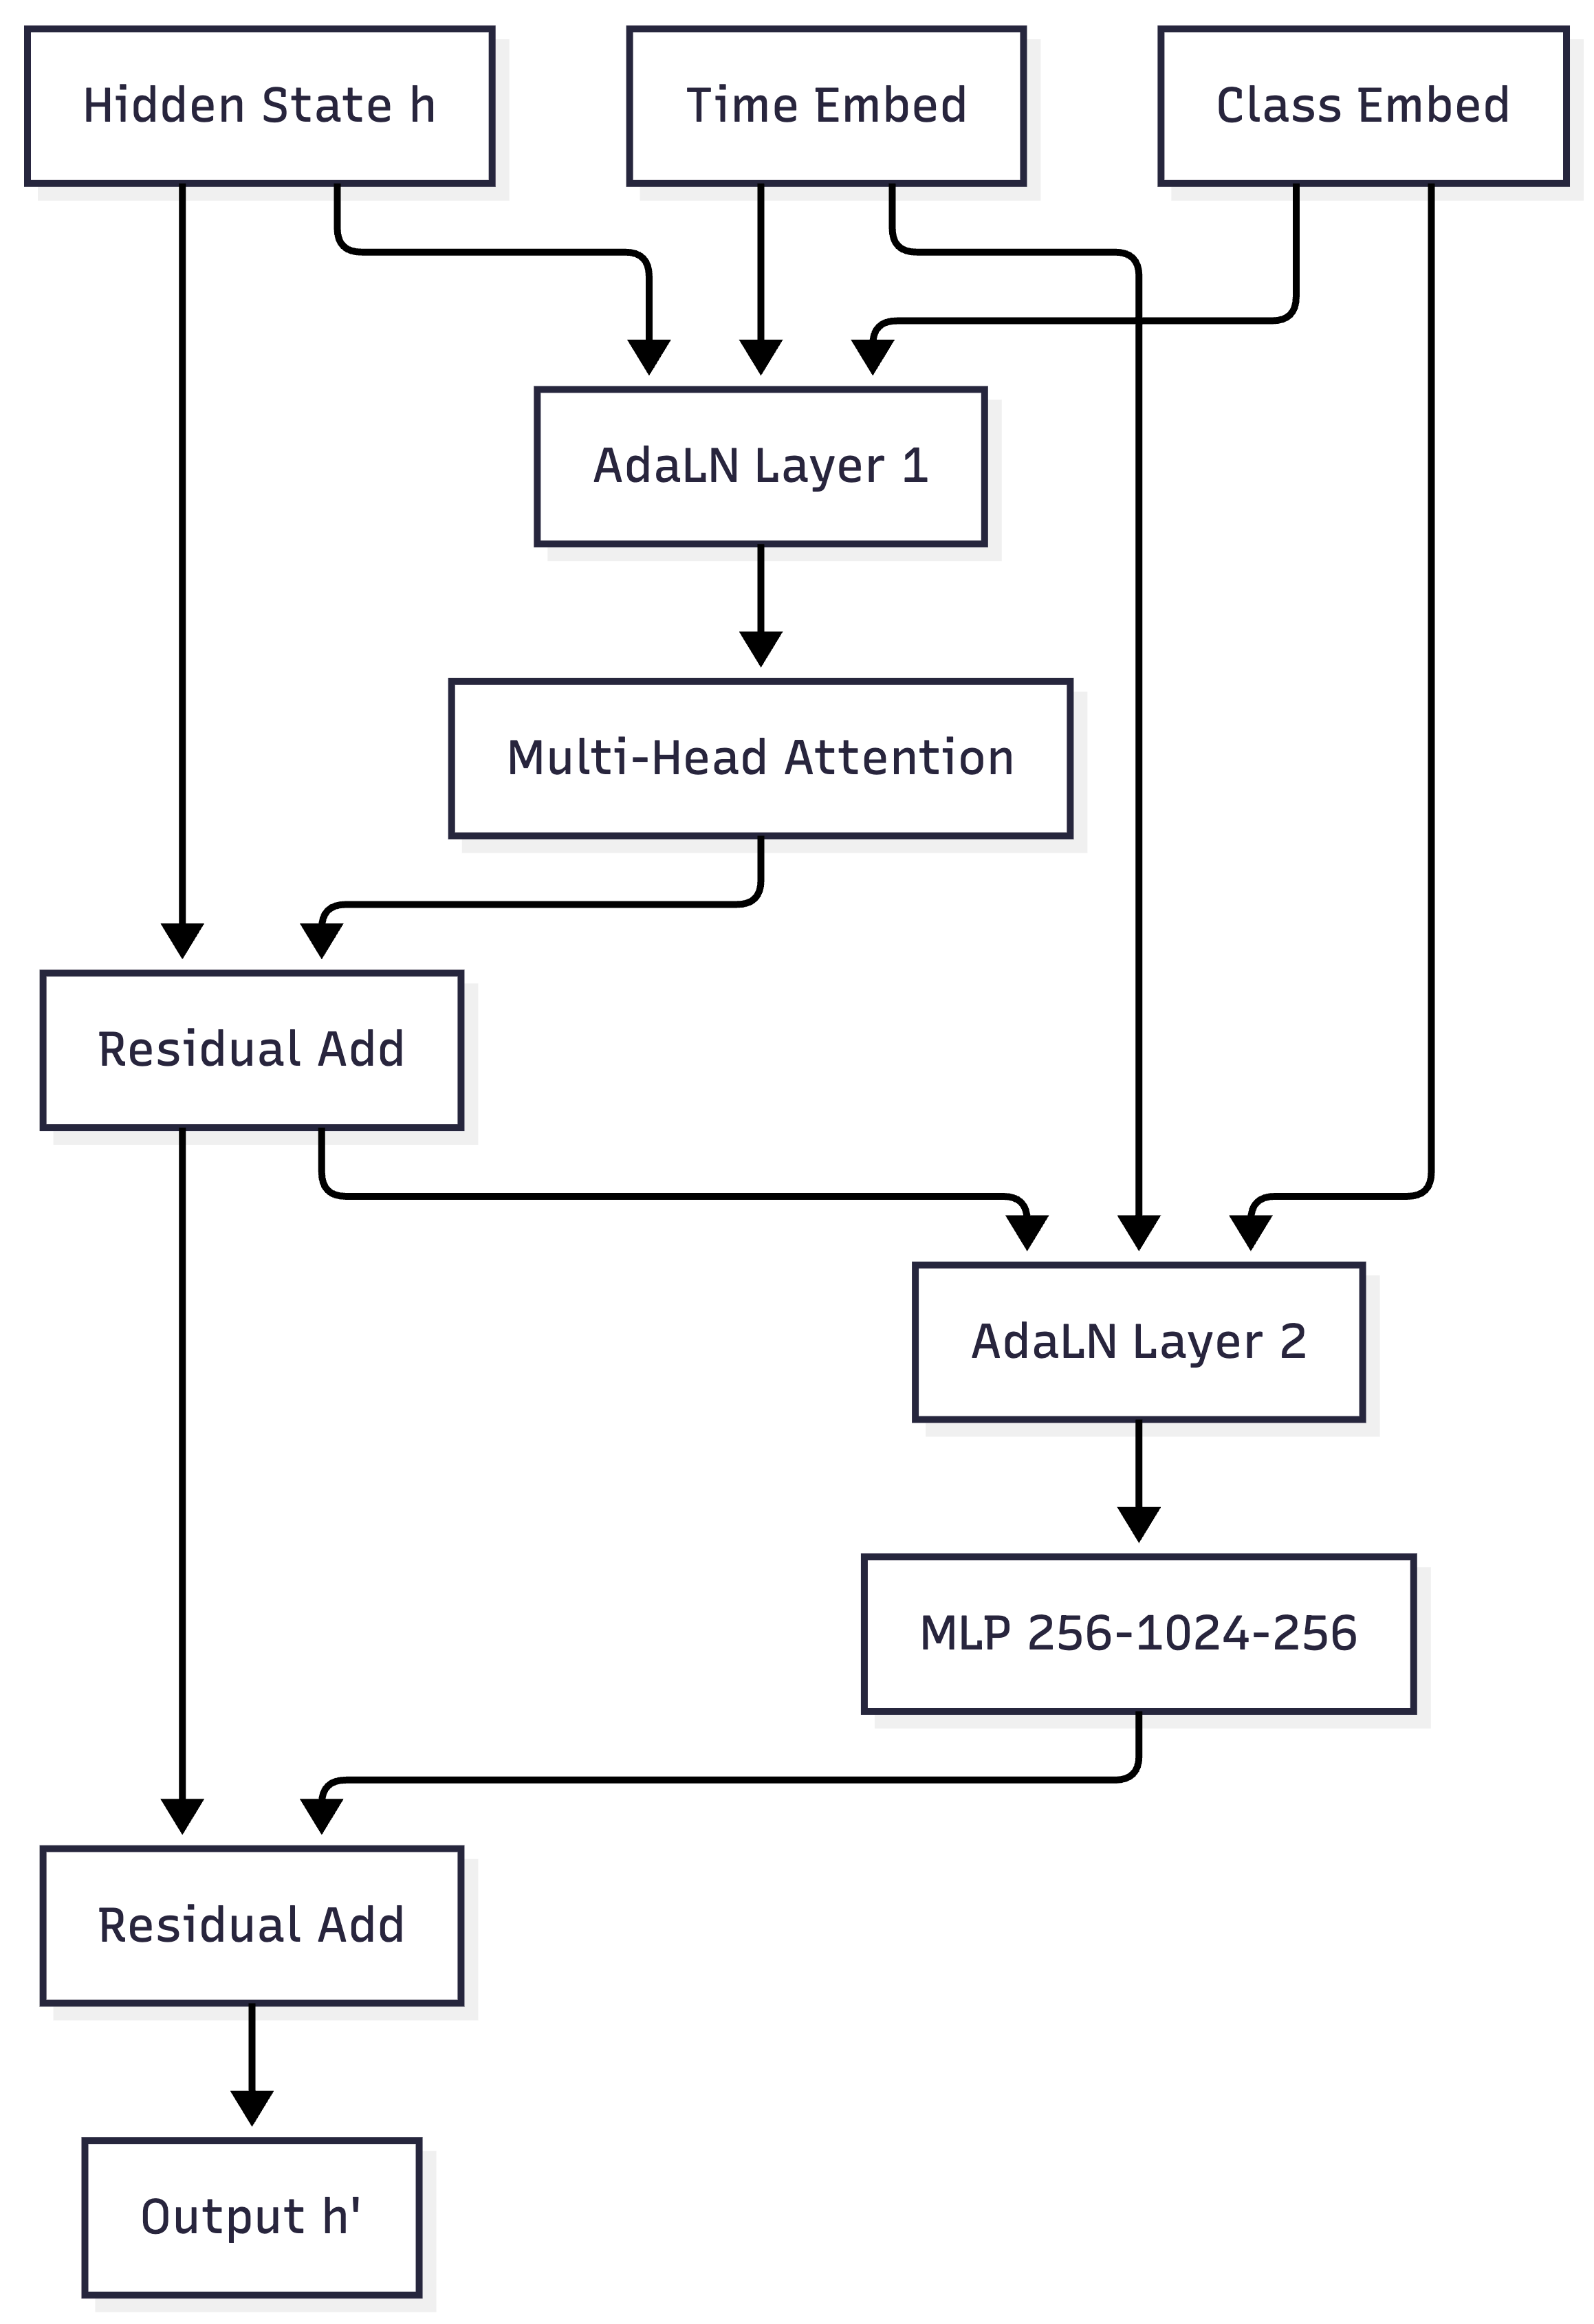
\includegraphics[width=0.45\textwidth]{img/dit_block.png}
\caption{Single DiT block with AdaLN conditioning.}
\label{fig:dit_block}
\end{figure}

The training objective minimizes the expected squared error between the true noise and the predicted noise:
\begin{equation}
\mathcal{L}_{diff} = \mathbb{E}_{t \sim \mathcal{U}(1,T),\, \mathbf{z}_0,\, \boldsymbol{\epsilon} \sim \mathcal{N}(\mathbf{0}, \mathbf{I})} \left[ \|\boldsymbol{\epsilon} - \epsilon_\theta(\sqrt{\bar{\alpha}_t}\,\mathbf{z}_0 + \sqrt{1-\bar{\alpha}_t}\,\boldsymbol{\epsilon},\, t,\, y)\|^2 \right]
\end{equation}

\subsection{Component 3: Classifier-free guidance}

Classifier-Free Guidance \cite{ho2022cfg} enables controllable generation in RE-TabSyn. The mechanism is illustrated in Figure~\ref{fig:cfg_mechanism}.

\begin{figure}[H]
\centering
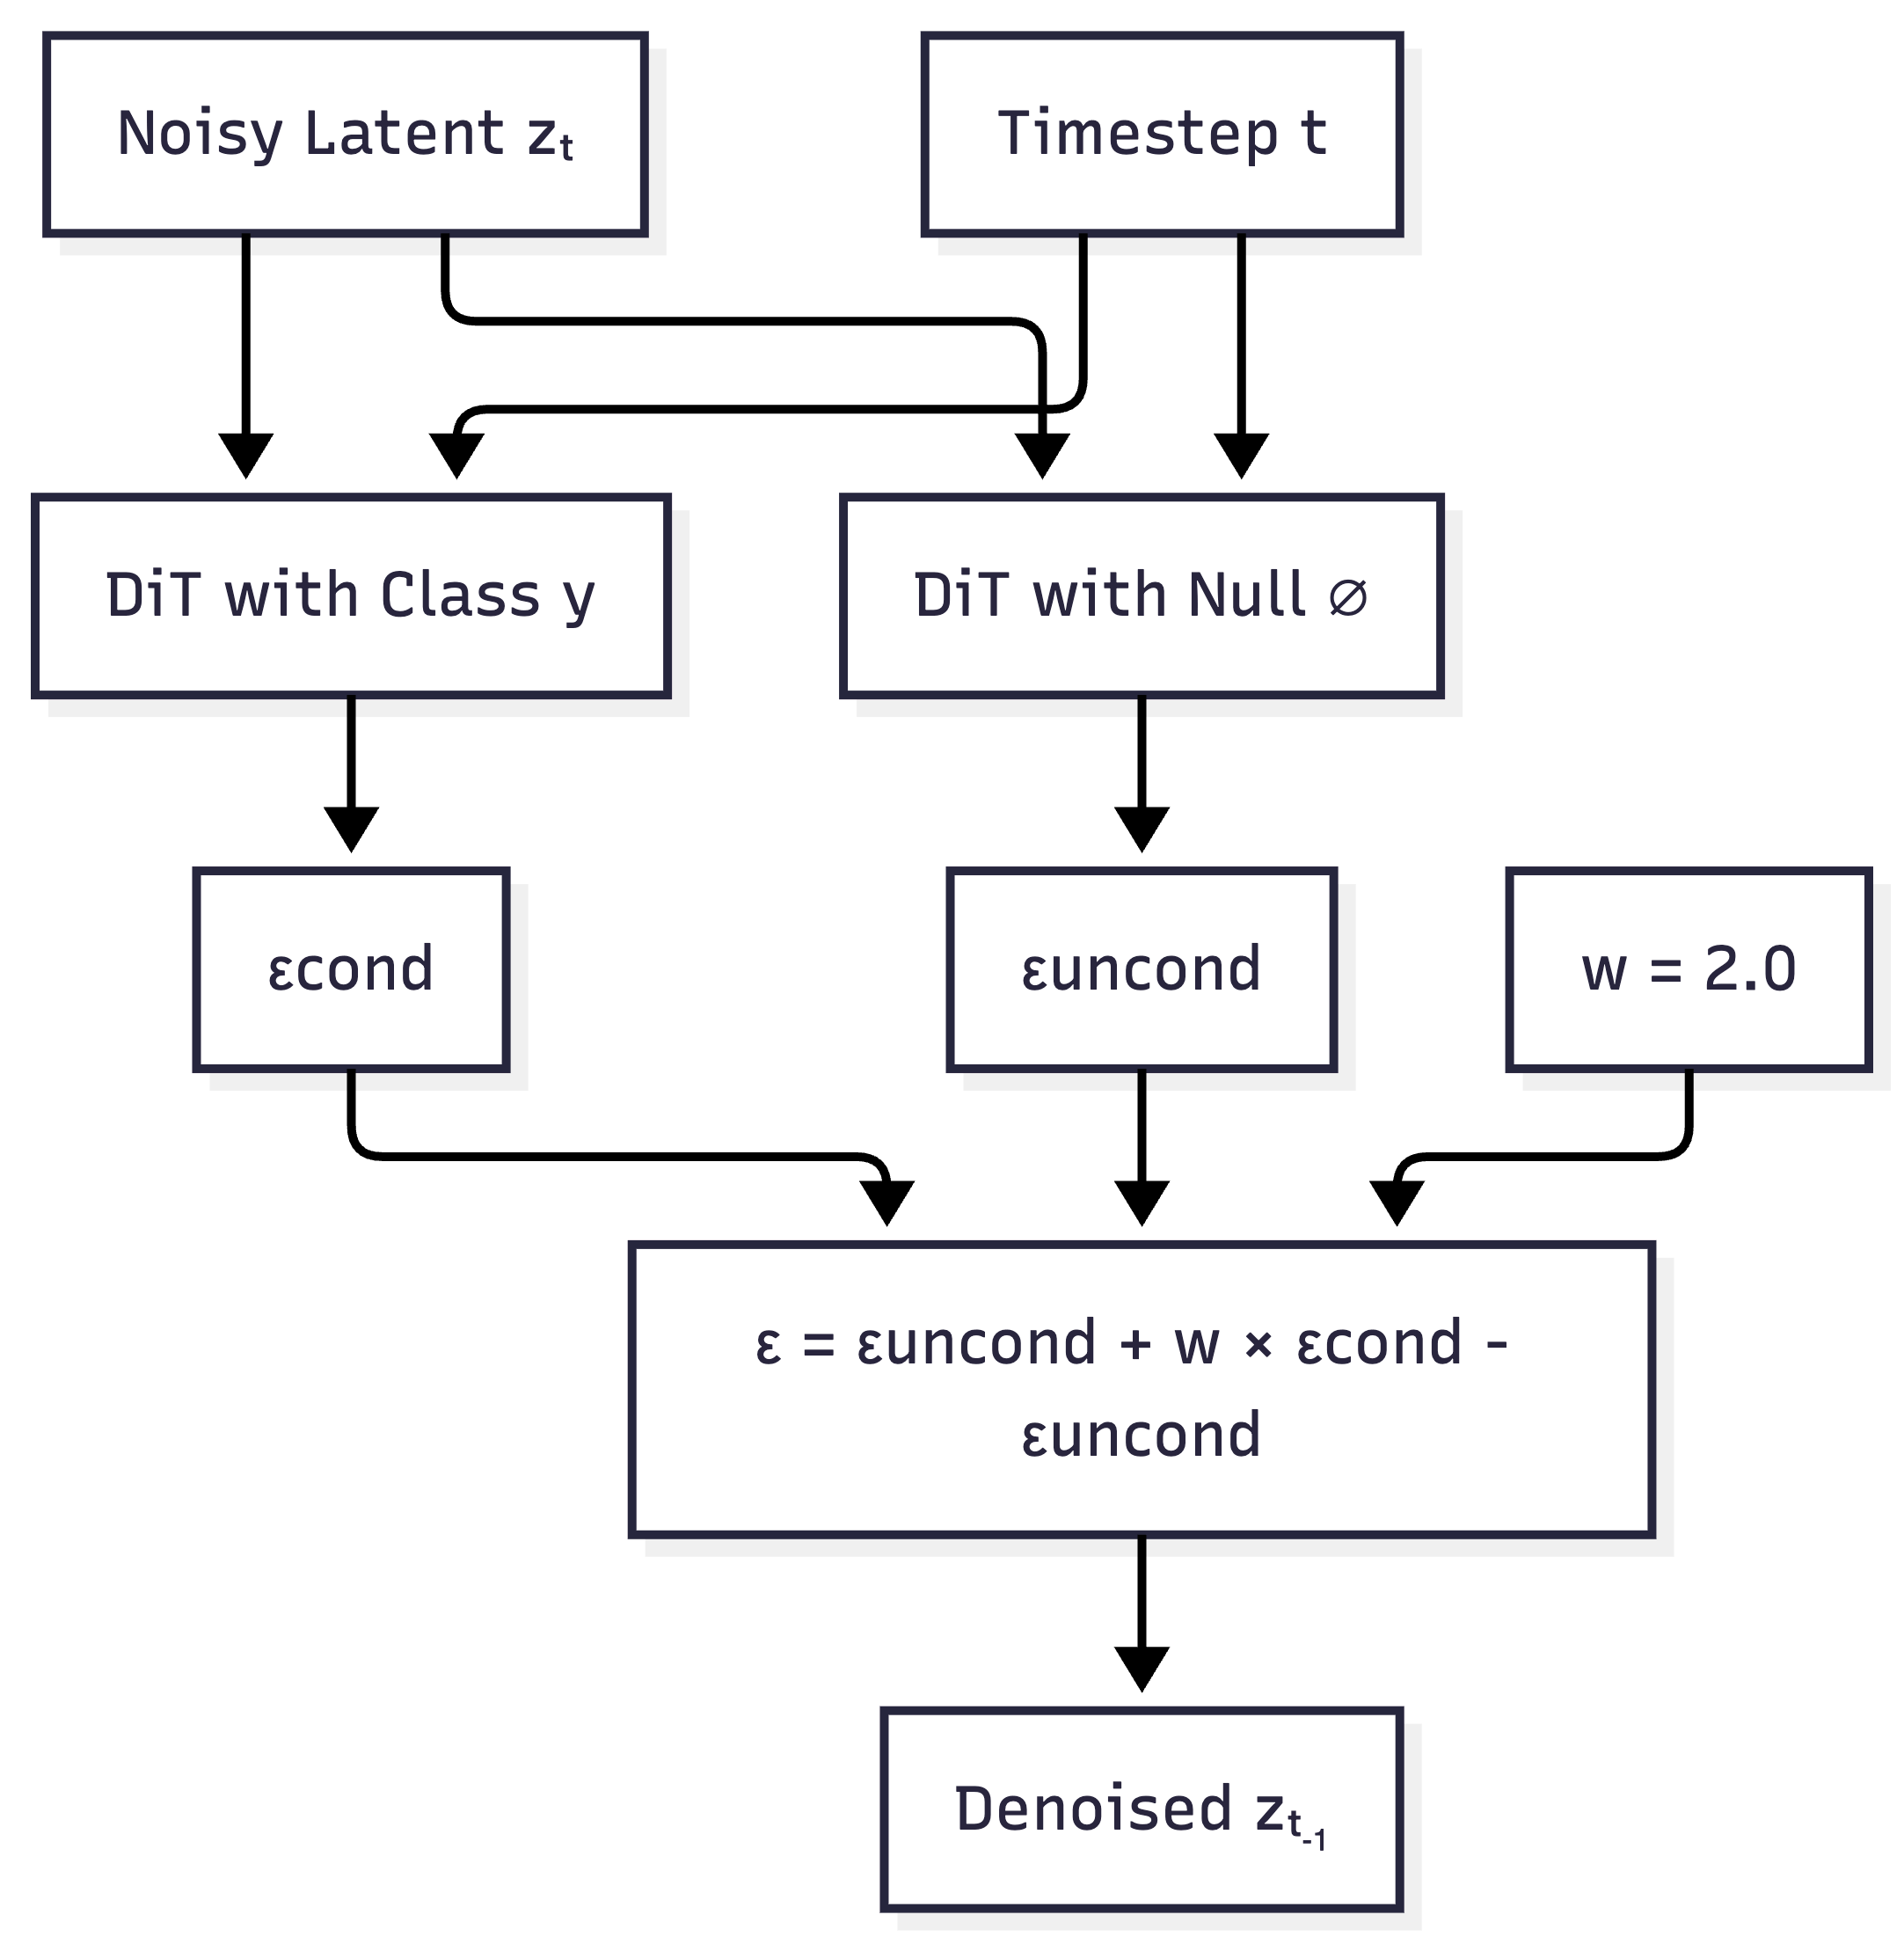
\includegraphics[width=0.7\textwidth]{img/cfg_mechanism.png}
\caption{CFG inference: two DiT passes blended.}
\label{fig:cfg_mechanism}
\end{figure}

During training, class labels are randomly replaced with a null token $\emptyset$ with probability $p_{uncond} = 0.10$, following the recommendation \cite{ho2022cfg}.

\begin{figure}[H]
\centering
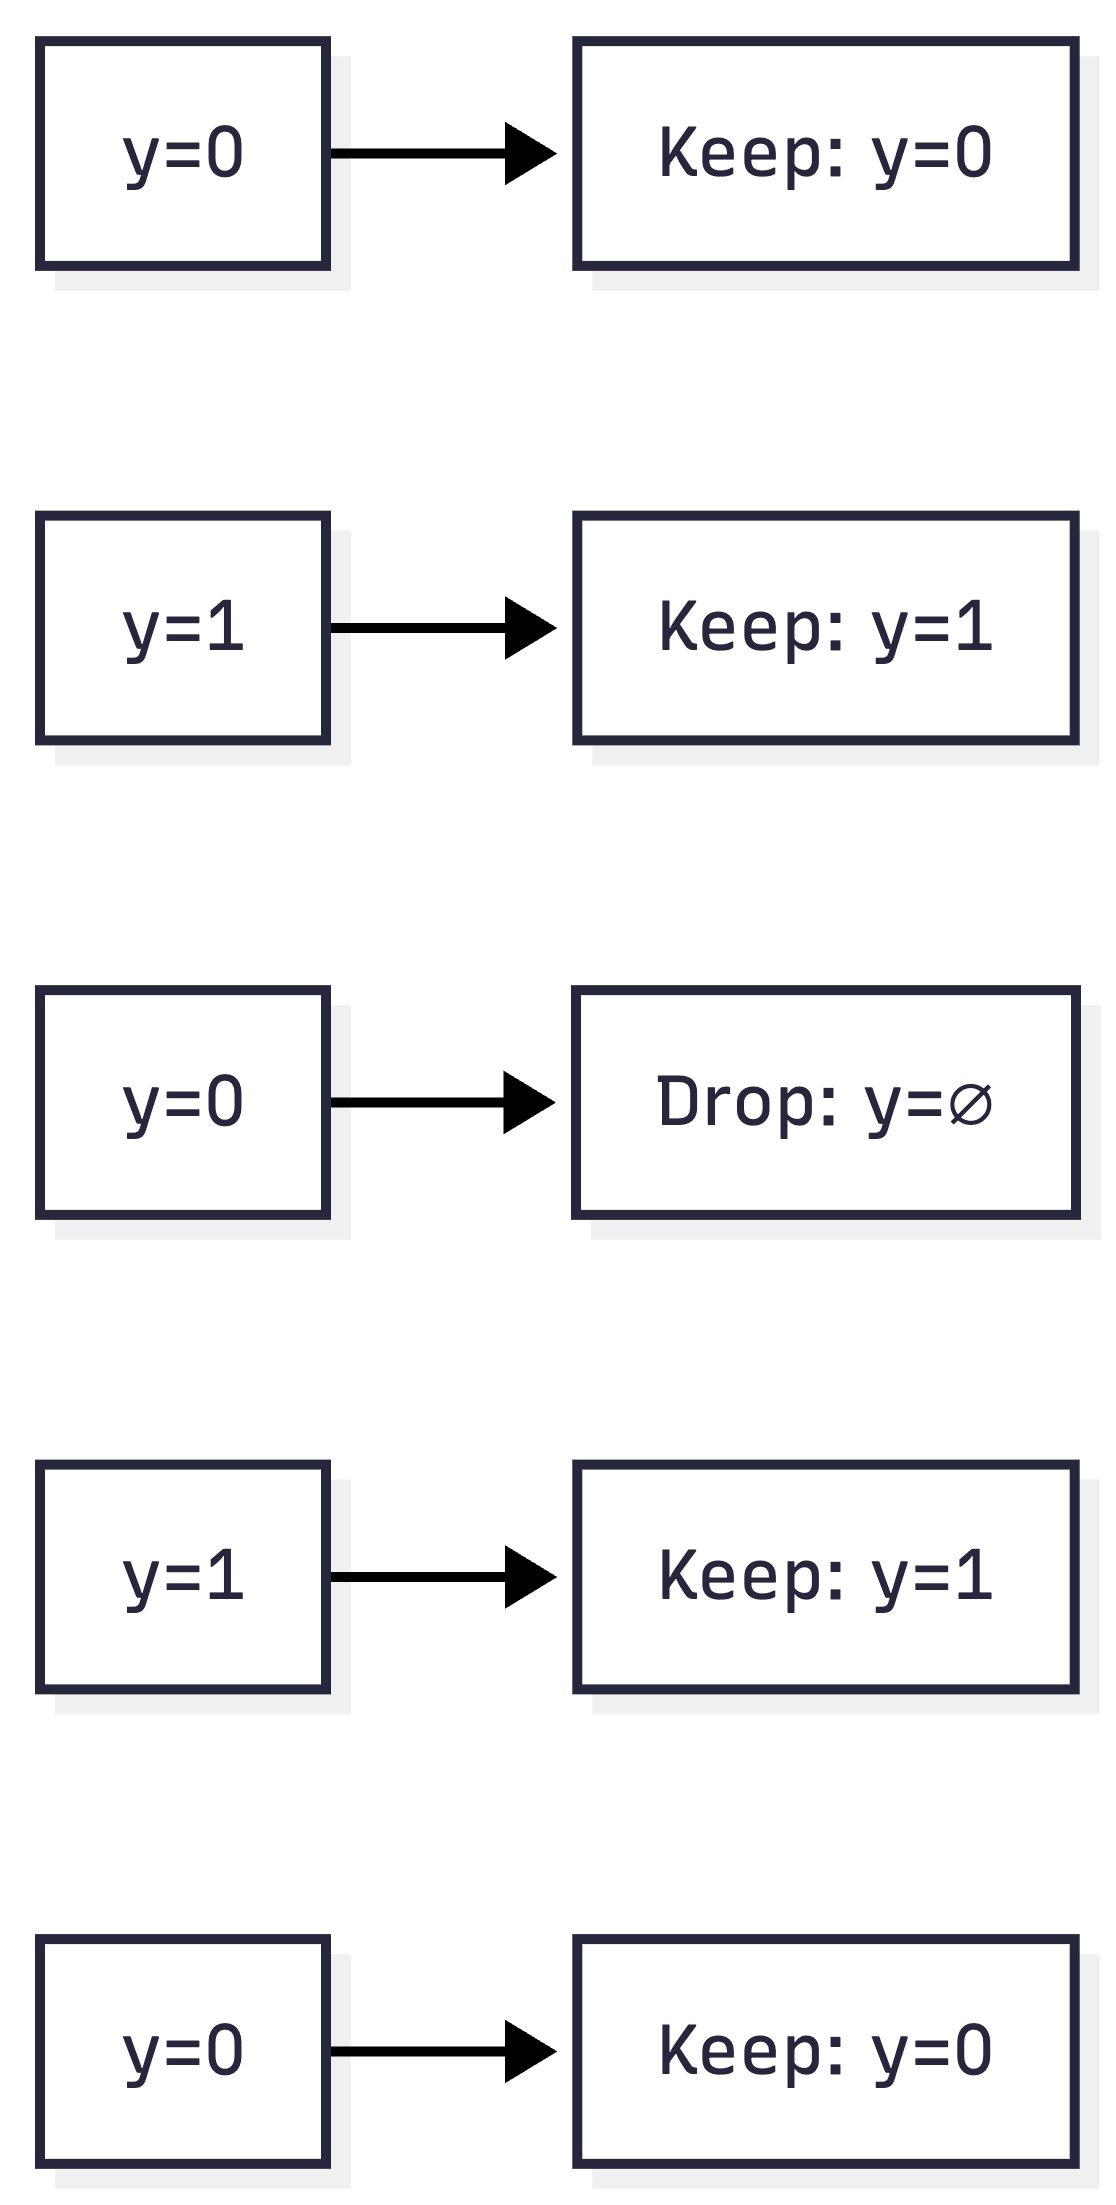
\includegraphics[width=0.4\textwidth]{img/cfg_label_dropout.png}
\caption{CFG label dropout (10\%) during training.}
\label{fig:cfg_label_dropout}
\end{figure}

This training procedure means the model simultaneously learns the conditional distribution $\epsilon_\theta(\mathbf{z}_t, t, y)$ and the unconditional distribution $\epsilon_\theta(\mathbf{z}_t, t, \emptyset)$.

At inference time, two forward passes are made for each denoising step. The noise predictions are interpolated (or extrapolated when $w > 1$):
\begin{equation}
\tilde{\epsilon}_\theta(\mathbf{z}_t, t, y) = \epsilon_\theta(\mathbf{z}_t, t, \emptyset) + w \cdot \left(\epsilon_\theta(\mathbf{z}_t, t, y) - \epsilon_\theta(\mathbf{z}_t, t, \emptyset)\right)
\end{equation}
where $w \geq 0$ is the guidance scale. At $w = 0$, generation is unconditional. At $w = 1$, it is standard conditional generation. The default $w = 2.0$ amplifies the class signal, producing near-50\% minority ratios (avg 1.1\% deviation from target) while maintaining KS = 0.163.

\section{Theoretical Analysis}

The two subsections below analyze why CFG works as a guidance mechanism for class control, and what the distributional cost of that control is in formal terms.

\subsection{Rationale for classifier-free guidance}

The rationale for CFG lies in its modification of the effective score function. Diffusion models learn the score function $\nabla_\mathbf{z} \log p(\mathbf{z})$, which points toward increasing data density. For class-conditional generation, the score should point toward regions of high density for the minority class specifically.

For a minority class $y = 1$, the guided score function becomes:
\begin{equation}
\nabla_{\mathbf{z}} \log \tilde{p}(\mathbf{z} | y=1) = (1-w) \nabla_{\mathbf{z}} \log p(\mathbf{z}) + w \nabla_{\mathbf{z}} \log p(\mathbf{z}|y=1)
\end{equation}

This is a linear combination of the unconditional score (pointing toward generally high-density regions) and the conditional score (pointing toward regions of high density for class 1). When $w = 2$, the guided score is $-\nabla_{\mathbf{z}} \log p(\mathbf{z}) + 2\nabla_{\mathbf{z}} \log p(\mathbf{z}|y=1)$: it moves away from generic high-density regions and doubly toward minority-class high-density regions.

This effectively samples from a reweighted (``sharpened'') distribution:
\begin{equation}
\tilde{p}(\mathbf{z} | y=1) \propto p(\mathbf{z})^{1-w} \cdot p(\mathbf{z}|y=1)^w
\end{equation}

When $w > 1$, probability mass concentrates in regions where $p(\mathbf{z}|y=1)$ is high relative to $p(\mathbf{z})$ --- the regions corresponding to minority class features. The guidance scale $w$ provides continuous, inference-time control over class bias without retraining.

\subsection{The fidelity-control trade-off}

Increasing $w$ boosts minority representation but introduces a distributional shift: the guided distribution $\tilde{p}$ deviates further from the true data distribution as $w$ increases.

This manifests as a modest increase in KS statistics from 0.109 (TabSyn, no guidance) to 0.163 (RE-TabSyn, $w = 2.0$) in our experiments, an increase of 0.054 in distributional distance. This is the trade-off between controllability and pure distributional fidelity.

Whether this trade-off is acceptable depends entirely on the application. For a practitioner trying to train a better fraud detection model, the relevant question is not ``is the KS statistic as low as possible?'' but ``does training on this synthetic data produce a better fraud detector than training on the original imbalanced data?'' The answer, as shown in Chapter~5, is yes: RE-TabSyn's balanced synthetic data produces a minority F1-score of 0.472, compared to 0.458 when training on the real imbalanced data. The small fidelity cost buys a measurable improvement in the task that matters.

As illustrated in Figure~\ref{fig:tradeoff}, RE-TabSyn maintains competitive fidelity while gaining class control. None of the baseline methods offer both properties simultaneously.

\begin{figure}[H]
\centering
\includegraphics[width=0.5\textwidth]{img/tradeoff.png}
\caption{Fidelity-control trade-off for RE-TabSyn.}
\label{fig:tradeoff}
\end{figure}

\section{Design Decisions Summary}

Table~\ref{tab:design_decisions} consolidates the architectural decisions in RE-TabSyn and the problem each one addresses. Twelve choices were made across the VAE, diffusion backbone, guidance mechanism, and training procedure. Each was driven by a concrete failure observed in preliminary experiments or in the baseline methods --- the table shows both what was chosen and what was rejected.

\renewcommand{\arraystretch}{1.2}

\begin{xltabular}{\textwidth}{|X|X|X|}
\caption{Architectural design decisions and rationale}
\label{tab:design_decisions} \\

\noalign{\hrule height\arrayrulewidth}
\textbf{Design Choice} & \textbf{Problem It Solves} & \textbf{Alternative Considered and Why Rejected} \\
\hline
\noalign{\vskip 4pt}
\hline
\endfirsthead

\noalign{\hrule height\arrayrulewidth}
\textbf{Design Choice} & \textbf{Problem It Solves} & \textbf{Alternative Considered and Why Rejected} \\
\hline
\noalign{\vskip 4pt}
\hline
\endhead

\hline
\multicolumn{3}{r}{\small\itshape Continued on next page} \\
\endfoot

\hline
\endlastfoot

VAE latent space & One-hot encoding is incompatible with continuous diffusion noise & Direct one-hot diffusion (TabDDPM): fails because noise on sparse binary vectors creates non-categorical intermediates \\
\hline
64-dimensional latent & Match largest dataset (Polish Bankruptcy, 64 features) & Smaller (32-d) reduces capacity; larger (128-d) adds training instability on small datasets \\
\hline
MLP encoder [256, 128] & Compact feature compression with stable gradients & Transformer encoder: better quality but considerably higher training cost; deferred to future work \\
\hline
$\beta = 0.1$ KL weight & Prevents posterior collapse without over-regularizing & $\beta = 1.0$ (standard VAE): causes posterior collapse on small datasets; $\beta = 0.01$: insufficient regularization \\
\hline
DiT Transformer backbone & Models inter-feature correlations via self-attention & MLP backbone (TabDDPM): cannot capture inter-feature dependencies; worse correlation preservation \\
\hline
4 DiT layers, dim 256 & Balance capacity and overfitting risk for datasets up to 45K rows & More layers: overfitting on small datasets; fewer layers: insufficient capacity \\
\hline
$T = 1000$ timesteps & Smooth noise trajectory for stable training and generation & $T = 100$: too coarse, worse quality; $T = 2000$: no quality gain, noticeably slower generation \\
\hline
Linear $\beta$ schedule & Proven stable across diverse datasets & Cosine schedule: marginally better for images, no benefit observed for tabular data \\
\hline
CFG ($p_{uncond} = 0.10$) & Enables class ratio control without auxiliary classifier & Classifier guidance: requires a separately trained classifier; couples generation to classification model quality \\
\hline
Guidance scale $w = 2.0$ & Near-50\% minority ratio with acceptable fidelity cost & Higher $w$ ($>$3): overshoots 50\% and degrades fidelity; lower $w$ ($<$1): insufficient minority boost \\
\hline
Two-phase training & Decouples representation learning from generative modeling & Joint training: latent space instability degrades both objectives simultaneously \\
\hline
Frozen VAE in Phase 2 & Prevents latent space drift during diffusion training & Unfrozen VAE: latent space changes invalidate already-trained diffusion parameters \\
\hline

\end{xltabular}

A consolidated reference for all mathematical symbols used in this chapter is provided in the Mathematical Notation section, immediately after the List of Abbreviations.
